% !TeX spellcheck = en_US
\section{Approach}
In the following we present the details of our approach.
\subsection{Dataset}
We used both of the DAVIS datasets \cite{davis_2016, davis_2017}, . These datasets include videos with segmentation ground truths for every frame. We trained on DAVIS17, as it contains more video sequences, but evaluated on DAVIS16, which is a subset of DAVIS17, since there only exists one annotation per frame. %TODO do we need explanation?
\subsection{Network Design}
Our architecture mainly uses MaskRCNN, which we extended with a SlowFast module between the backbone and the head. An overview is shown in   Fig.~\ref{architecture}. The backbone is a ResNet50 Feature Pyramid Network, which was pretrained on Coco %TODO cite 
and fine-tuned on DAVIS17 \cite{davis_2017}.

The computed feature maps of several frames are fed into the SlowFast module, which can be seen in Fig.~\ref{slowfast}. It consists of two pathways, both with three 3D convolutions, followed by batch norm and for the first two layers a ReLu activation. After the first two layers the outputs of the fast pathway are fused into the slow pathway using another combination of Convolution, Batchnorm and ReLu.

The final outputs of the slow and the fast pathway are then concatenated and used as input for the Mask R-CNN head. Additionally the head also receives region proposals computed by a RPN, which works with the original image features computed by the backbone.

\begin{figure}
	\centering
	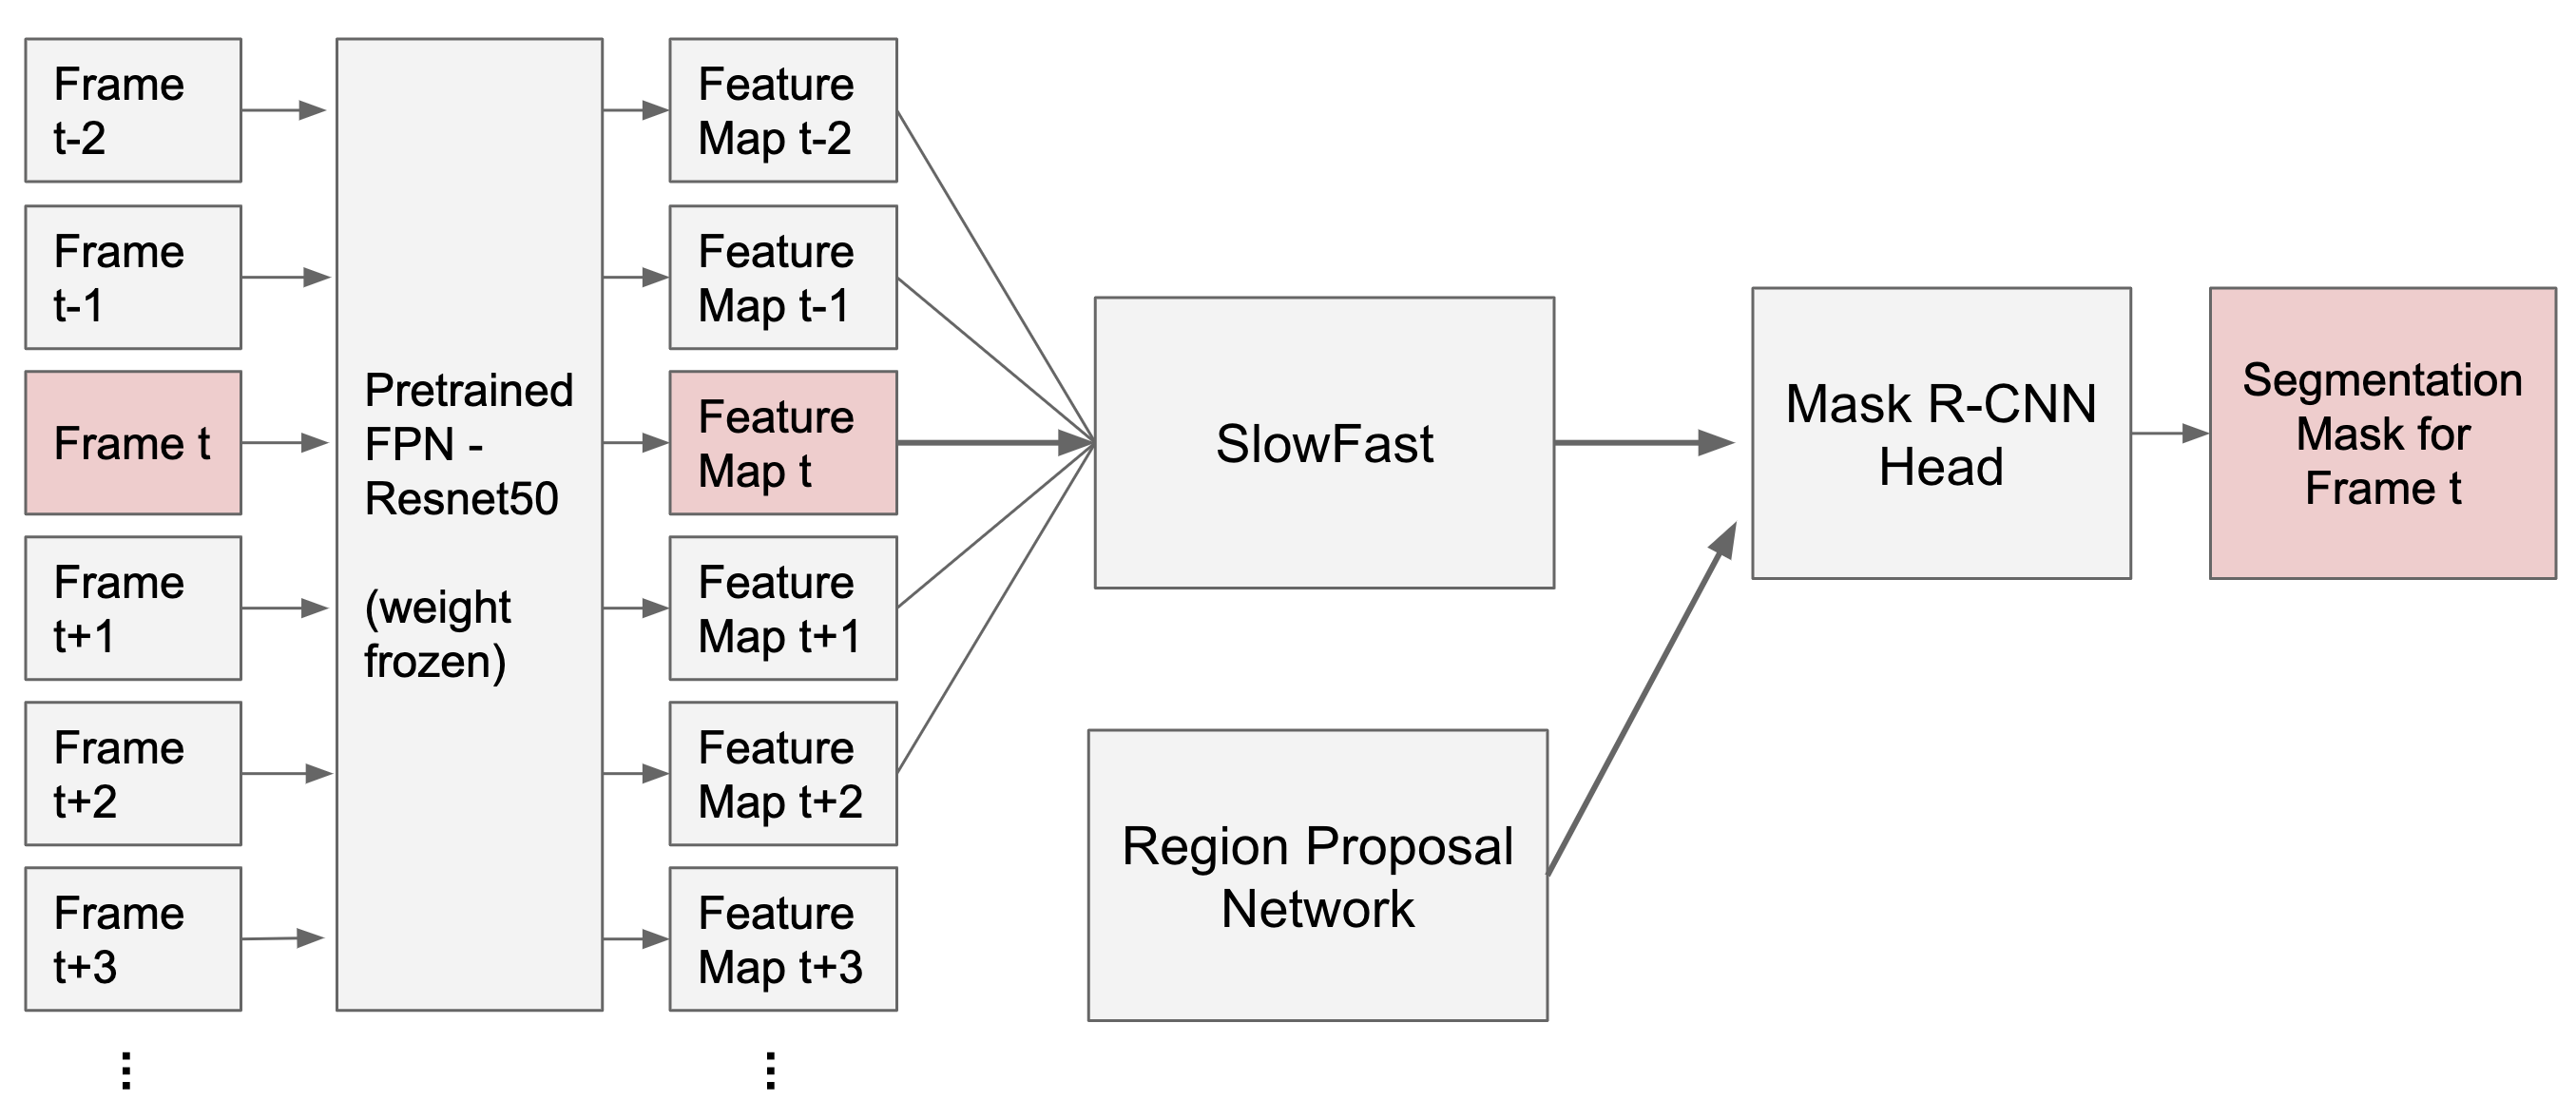
\includegraphics[width=\columnwidth]{figures/architecture.png}
	\caption{Architecture Overview.}
	\label{architecture}
\end{figure}

\begin{figure}
	\centering
	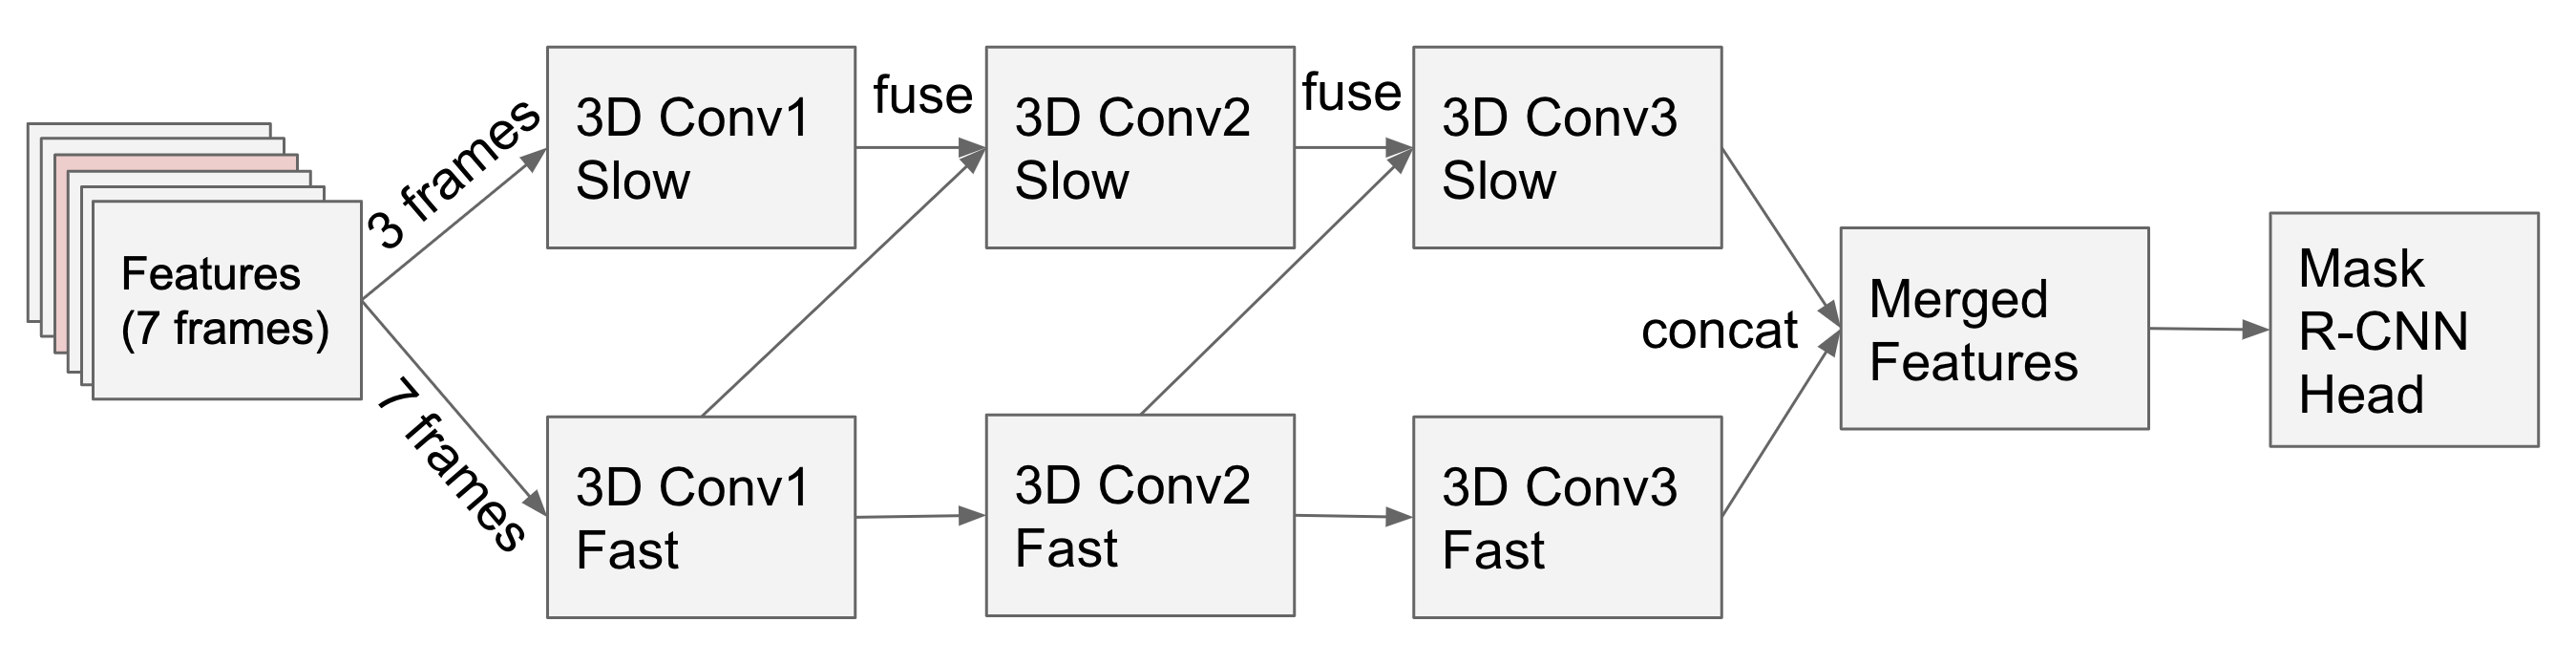
\includegraphics[width=\columnwidth]{figures/slowfast.png}
	\caption{Overview of SlowFast Layers.}
	\label{slowfast}
\end{figure}
\subsection{Training}
For the unsupervised case we are training for 20 epochs on the training data of DAVIS17 \cite{davis_2017}. We are using SGD with momentum as optimizer and our learning rate is set to 0.0001.

The semi-supervised training starts with a parent model trained on the task of unsupervised VOS and finetunes this model on specific sequences, resulting in one model per sequence. We are using different augmentations, including Random Horizontal Flip, Rotation of up to 30 degrees, and Scaling of the image. We experimented with different scaling strengths and learning rates, that are described in the experiment section.